\documentclass[conference]{IEEEtran}
\IEEEoverridecommandlockouts
\usepackage{cite}
\usepackage{amsmath,amssymb,amsfonts}
\usepackage{graphicx}
\usepackage{textcomp}
\def\BibTeX{{\textrm{B}\kern-.05em{\textsc{i\kern-.025em b}}\kern-.08em
    T\kern-.1667em\lower.7ex\hbox{E}\kern-.125emX}}

\begin{document}

\title{Distributed Large Language Model Inference Serving via Layer-Wise Pipeline Parallelism}

\author{\IEEEauthorblockN{Wiratmika}
\IEEEauthorblockA{University of Washington \\
Tacoma, WA, United States \\
wmika@uw.edu}}

\maketitle

\begin{abstract}
Large language model (LLM) inference is increasingly constrained by memory footprint and end-to-end latency, especially when deployment hardware is limited to commodity CPU virtual machines. This project studies whether layer-wise pipeline model parallelism over HTTP can make distributed inference practical in such constrained environments, and where communication overhead dominates potential compute gains. We implement a complete gateway-worker serving stack for GPT-2 Medium (355M) with contiguous layer sharding across 1, 2, and 4 nodes, instrumenting per-stage compute, serialization, network hop time, memory, time-to-first-token (TTFT), and end-to-end latency. Evaluation is performed on cloud VMs using 15 benchmark configurations spanning prompt lengths (32, 128, 512 tokens) and client concurrency (1, 2, 3), each with warmup and repeated measurements. Results show that in this implementation distributed execution consistently increases single-request latency (up to 77.1\% at 4 nodes for 128-token prompts), while the network share of wall-clock time ranges from 17.2\% to 51.6\% across configurations and grows with node count, indicating communication-bound behavior under the tested setup.
\end{abstract}

\begin{IEEEkeywords}
Distributed inference, large language models, pipeline parallelism, model sharding, serving systems, performance evaluation
\end{IEEEkeywords}

\section{Introduction}
Large language models have grown faster than the memory and compute budgets typically available on a single commodity machine. A common response is model parallelism, where layers are partitioned across devices and intermediate activations are transferred between them. In production settings this can unlock larger models, but it also introduces communication and synchronization costs that may cancel out theoretical speedups.

This work investigates a concrete systems question: \textit{for CPU-only inference, when does simple layer-wise pipeline partitioning over HTTP help, and when does it hurt?} The project implements a full distributed serving prototype rather than simulation, with a FastAPI gateway orchestrating autoregressive decoding and worker nodes executing contiguous transformer layer shards.

The implementation emphasizes observability. In addition to standard latency and throughput metrics, the system records per-node compute and serialization times, estimated network-hop delays, TTFT, and peak RSS memory. This instrumentation supports causal diagnosis (compute-bound vs. communication-bound regimes) instead of reporting aggregate latency alone.

The implemented and benchmarked configuration uses GPT-2 Medium, node counts \{1,2,4\}, prompt lengths \{32,128,512\}, and concurrency levels \{1,2,3\}.

\section{Research Questions}
The evaluation is organized around the following research questions:

\begin{itemize}
\item \textbf{Scaling under single-client load}: How do latency and TTFT change as node count increases from 1 to 2 to 4?
\item \textbf{Time breakdown}: What fraction of end-to-end latency is attributable to network transfer versus model compute?
\item \textbf{Concurrency behavior}: Does higher request concurrency improve system-level throughput enough to offset distributed overhead?
\item \textbf{Input-length sensitivity}: How does prompt length influence the communication-to-compute ratio in distributed runs?
\item \textbf{Memory effects}: How does peak per-node memory change across different partitions?
\end{itemize}

\section{Related Work}
Pipeline and model parallel training systems such as GPipe~\cite{gpipe} and PipeDream~\cite{pipedream} established the core idea of splitting neural network layers across devices and overlapping execution. Megatron-LM~\cite{megatron} and GShard~\cite{gshard} expanded this design space with tensor and expert parallel strategies at larger scales.

For LLM serving, recent systems focus on improving throughput/latency trade-offs through specialized runtime techniques (e.g., KV-cache paging and continuous batching in vLLM~\cite{vllm}, or prefill/decoding disaggregation in DistServe~\cite{distserve}). These methods target high-performance GPU environments and often rely on optimized kernels, scheduling, and memory managers.

Our approach differs in goal and scope: we intentionally study a simpler CPU-only, HTTP-based, layer-partitioned deployment to expose first-order distributed systems trade-offs in an accessible environment. The novelty here is not a new parallel algorithm but an end-to-end reproducible prototype with fine-grained timing instrumentation that isolates where distributed overhead emerges in practice.

\section{Methodology}
\subsection{System Architecture}
The serving stack contains one gateway and multiple worker processes. The gateway accepts client requests, tokenizes prompts, and performs autoregressive decoding one token at a time. For each decoding step, it sends token IDs (for the initial prefill) to the rank-0 worker. That worker executes its layer shard and recursively forwards outputs through subsequent workers until the last stage returns logits to the gateway.

Each worker hosts a ModelShard containing a contiguous slice of GPT-2 Medium transformer blocks. Partitioning is static and rank-based. For \(N\in\{1,2,4\}\), workers are pre-provisioned with corresponding rank and next-hop routing.

\subsection{Communication and Serialization}
Inter-node communication uses HTTP/JSON with base64-encoded tensors for activation transport. This design favors implementation simplicity and deployment portability over raw performance, and intentionally makes serialization and network costs measurable.

\subsection{Instrumentation}
The implementation records:
\begin{itemize}
\item End-to-end latency and TTFT at the gateway.
\item Total network time estimated from request/response wall-clock hop timings.
\item Per-node compute and serialization time accumulated across decoding steps.
\item Peak per-node RSS memory.
\item Tokens generated and derived throughput.
\end{itemize}

\subsection{Experimental Design}
Two benchmark groups are implemented.
\begin{itemize}
\item \textbf{Scaling group:} nodes \(\in\{1,2,4\}\), input length \(\in\{32,128,512\}\), concurrency \(=1\).
\item \textbf{Concurrency group:} nodes \(\in\{1,2,4\}\), input length \(=128\), concurrency \(\in\{1,2,3\}\).
\end{itemize}
All runs use GPT-2 Medium, generation length 50, one warmup run, and repeated measurements written to JSON.

\section{Evaluation}
\subsection{Platform and Setup}
Experiments are deployed on Google Cloud VMs (Ubuntu 22.04, machine type c4d-highmem-2). A pool of one gateway and seven worker instances is provisioned so that 1-node, 2-node, and 4-node logical pipelines can each be realized from dedicated workers without redeployment. Inference uses CPU only.

\subsection{Practical Constraints and Scope Adjustment}
The original plan targeted larger-model experiments, including GPT-2 XL, to more strongly test memory-pressure benefits of sharding. In practice, available instance options under the current account were limited, especially for high-memory-bandwidth CPUs. Under these constraints, large-model distributed runs encountered frequent end-to-end timeouts even with relaxed timeout settings. To complete the study within feasible runtime and budget limits, the model was reduced to GPT-2 Medium while preserving the same factor-based experiment design (node scaling, input-length scaling, and concurrency scaling).

\subsection{Primary Results}
Figures~\ref{fig:latency_node_count} and~\ref{fig:ttft_node_count} show that increasing nodes consistently increases both end-to-end latency and TTFT for all prompt lengths. Relative to one node, two-node latency increases by 20.5\% (32-token), 27.3\% (128-token), and 24.9\% (512-token). Four-node latency increases by 60.2\%, 77.1\%, and 75.3\%, respectively. Under this implementation, added communication dominates reduced per-stage compute. Run-level variability is low (relative standard deviation $<$1.5\% across all configurations; see Tables~\ref{tab:latency_c1} and~\ref{tab:raw_variability} in the Appendix for exact values).

\begin{figure}[ht]
\centering
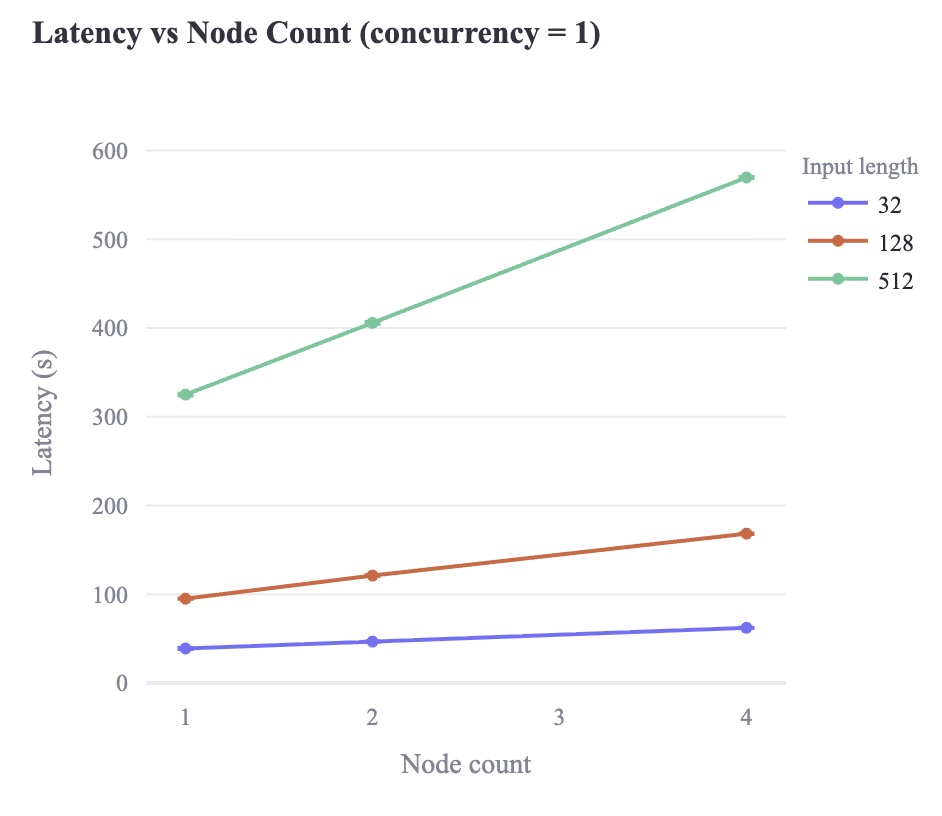
\includegraphics[width=\linewidth]{charts/1-latency-node-count.jpg}
\caption{Latency vs. node count per input length (32, 128, 512).}
\label{fig:latency_node_count}
\end{figure}

\begin{figure}[ht]
\centering
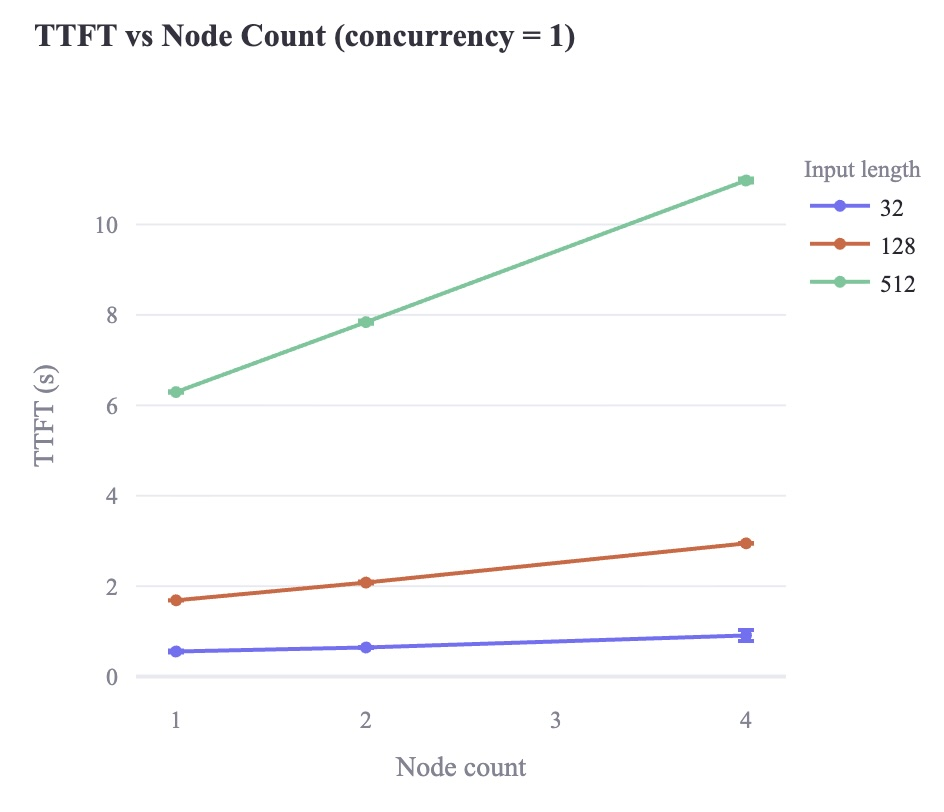
\includegraphics[width=\linewidth]{charts/2-ttft-node-count.jpg}
\caption{TTFT vs. node count per input length (32, 128, 512).}
\label{fig:ttft_node_count}
\end{figure}

\subsection{Communication vs. Compute Breakdown}
Figure~\ref{fig:time_share_breakdown} decomposes wall-clock time into four categories: model compute, serialization (encoding/decoding tensors), network transfer, and residual (gateway-side orchestration overhead such as token sampling, loop control, and Python scheduling not captured by the other three categories). Median network-time share increases sharply with node count:
\begin{itemize}
\item 1 node: 17.2--22.5\% (across input lengths)
\item 2 nodes: 29.7--36.0\%
\item 4 nodes: 45.0--51.6\%
\end{itemize}
Conversely, compute share decreases from roughly 68--77\% (1 node) to 39--48\% (4 nodes). This quantitatively supports the communication-bound diagnosis for multi-node runs. Precise per-configuration percentages are tabulated in Table~\ref{tab:raw_share} (Appendix).

\begin{figure}[ht]
\centering
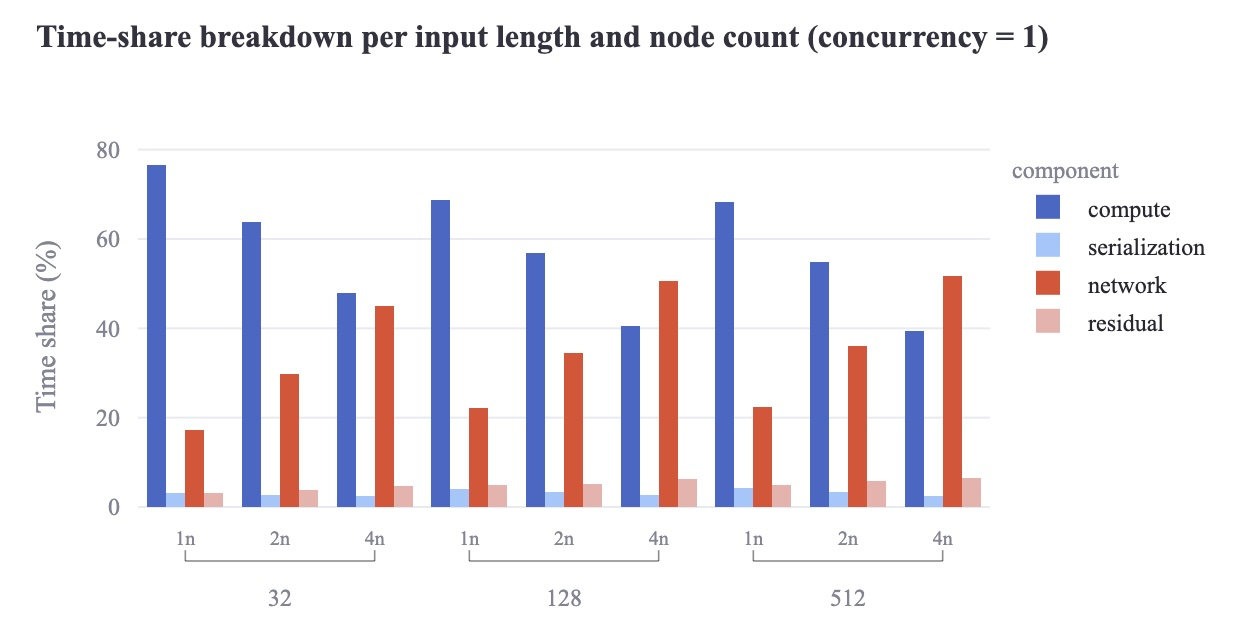
\includegraphics[width=\linewidth]{charts/3-time-share-breakdown.jpg}
\caption{Grouped wall-clock time-share decomposition (compute, serialization, network, residual) for each \{input length, node count\} configuration at concurrency 1.}
\label{fig:time_share_breakdown}
\end{figure}

\subsection{Concurrency Results}
Table~\ref{tab:throughput_concurrency} reports overall throughput for input length 128.

\begin{table}[ht]
\caption{System throughput (tokens/s) at input length 128}
\label{tab:throughput_concurrency}
\centering
\begin{tabular}{|c|c|c|c|c|}
\hline
Input tokens & Concurrency & 1 node & 2 nodes & 4 nodes \\
\hline
128 & 1 & 0.5259 & 0.4128 & 0.2970 \\
128 & 2 & 0.5397 & 0.4398 & 0.3553 \\
128 & 3 & 0.5363 & 0.5072 & 0.4874 \\
\hline
\end{tabular}
\end{table}

Higher concurrency narrows the throughput gap between node counts, but does not reverse ordering in this dataset: 1-node remains highest, while 4-node approaches 2-node at 3 concurrent clients. We therefore explicitly report a negative result: this implementation did not achieve higher throughput with increased node count. This suggests partial pipeline utilization gains under concurrency, but not enough to overcome communication and serialization costs.

\begin{figure}[ht]
\centering
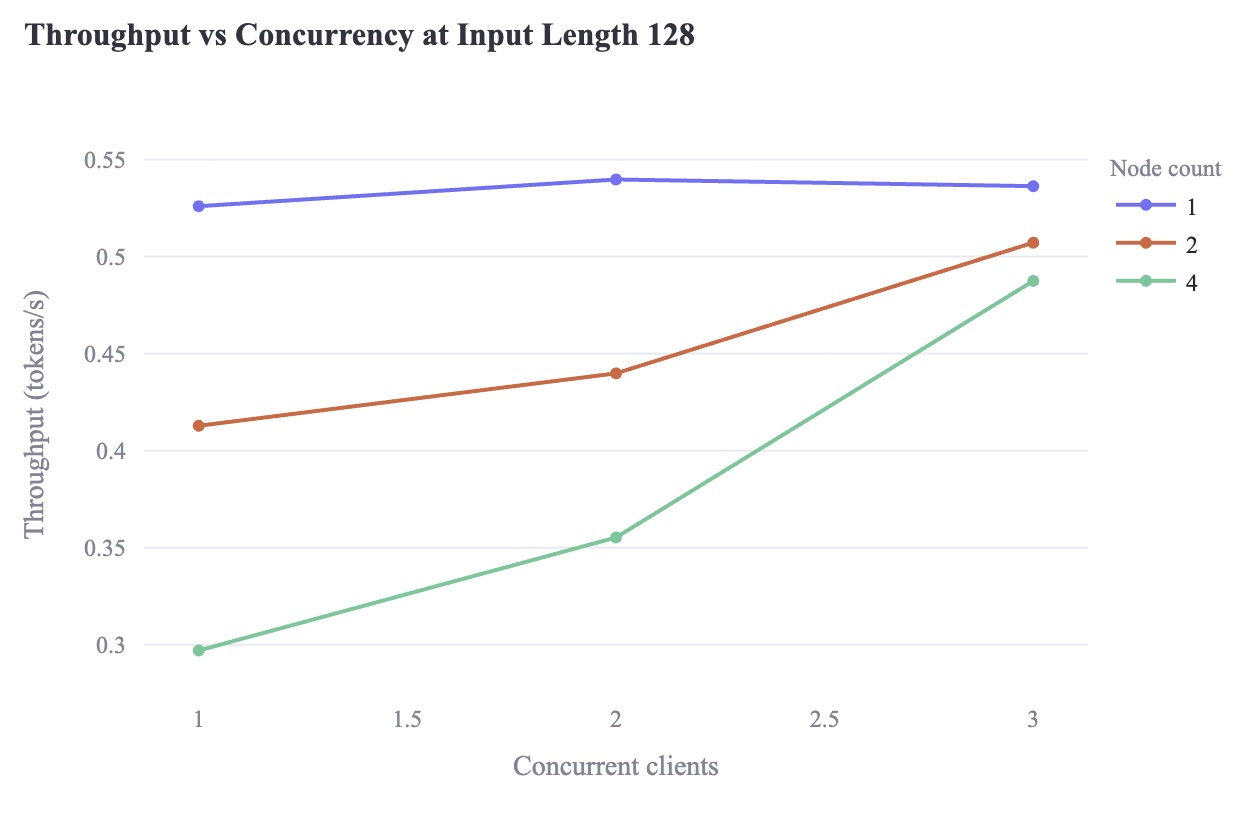
\includegraphics[width=\linewidth]{charts/4-throughput-concurrency.jpg}
\caption{Throughput vs. concurrency at input length 128 per node count.}
\label{fig:throughput_concurrency}
\end{figure}
Throughput deltas relative to the 1-node baseline (Table~\ref{tab:raw_tput_rel} in the Appendix) confirm that the deficit shrinks with concurrency but remains negative in all configurations.

\subsection{Memory Observations}
Peak RSS per node does not decrease monotonically with more shards in these runs; several first-stage workers show higher memory than expected under larger node counts. This likely reflects framework/runtime overhead, duplicated model components (e.g., embeddings/heads depending on shard placement), and Python process overhead. A deeper memory attribution study is needed before claiming linear sharding benefits.

\begin{figure}[ht]
\centering
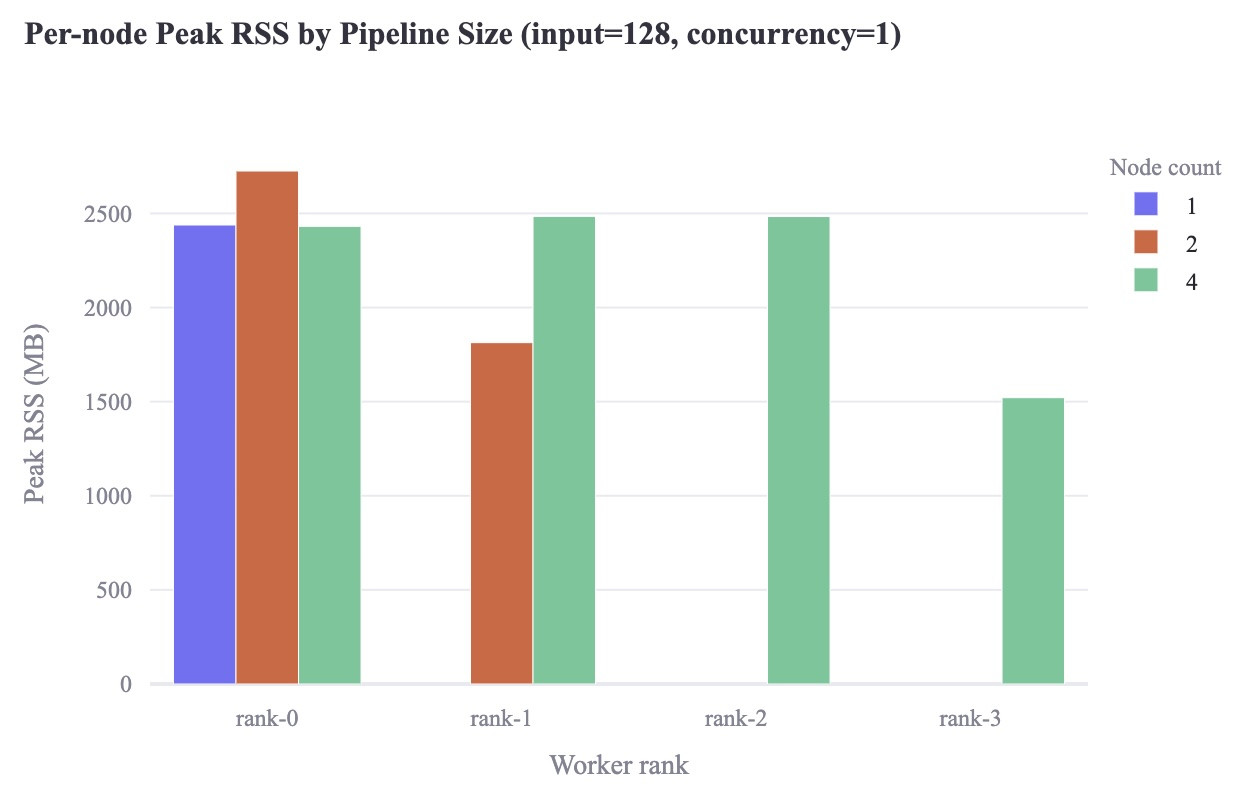
\includegraphics[width=\linewidth]{charts/5-per-node-peak-rss.jpg}
\caption{Per-node peak RSS across node counts 1, 2, and 4 for the representative setting (input length 128, concurrency 1).}
\label{fig:peak_rss}
\end{figure}

\section{Conclusion}
This project demonstrates an end-to-end distributed LLM inference prototype using layer-wise pipeline partitioning over HTTP in a CPU-only environment. The implementation successfully supports 1/2/4-node sharding, detailed telemetry, and reproducible benchmarking; however, measured performance indicates that communication and serialization overhead dominate benefits from parallel stage compute in the tested regime. Single-request latency increases with node count across all prompt lengths, and while higher concurrency narrows the throughput gap between node counts, it does not reverse the ordering. Critically, we did not achieve the originally hoped throughput scaling with additional nodes under this setup. The study should be interpreted as a constrained but practical baseline rather than a final verdict on distributed inference, since unavailable high-bandwidth instance classes and timeout pressure prevented the originally intended larger-model evaluation.

Future work should focus on code and infrastructure optimization: replacing the synchronous HTTP request-response forwarding with asynchronous fire-and-forget messaging so that communication is truly unidirectional and pipeline stages can overlap, reducing transport overhead (binary protocols, tensor compression, or shared-memory/RDMA options), improving scheduling and batching at the gateway, minimizing Python serialization overhead, and re-running the same protocol on larger models and stronger hardware to test whether conclusions change at greater scale.

\begin{thebibliography}{9}

\bibitem{gpipe}
Y. Huang, Y. Cheng, A. Bapna, et al.,
``GPipe: Efficient Training of Giant Neural Networks using Pipeline Parallelism,''
in \textit{Proc. NeurIPS}, 2019.

\bibitem{pipedream}
D. Narayanan, M. Harlap, A. Phanishayee, et al.,
``PipeDream: Generalized Pipeline Parallelism for DNN Training,''
in \textit{Proc. ACM SOSP}, 2019.

\bibitem{megatron}
M. Shoeybi, M. Patwary, R. Puri, et al.,
``Megatron-LM: Training Multi-Billion Parameter Language Models Using Model Parallelism,''
arXiv:1909.08053, 2019.

\bibitem{gshard}
D. Lepikhin, H. Lee, Y. Xu, et al.,
``GShard: Scaling Giant Models with Conditional Computation and Automatic Sharding,''
in \textit{Proc. ICML}, 2021.

\bibitem{vllm}
W. Kwon, Z. Li, S. Zhuang, et al.,
``Efficient Memory Management for Large Language Model Serving with PagedAttention,''
in \textit{Proc. ACM SOSP}, 2023.

\bibitem{distserve}
Y. Zhong, S. Liu, J. Li, et al.,
``DistServe: Disaggregating Prefill and Decoding for Goodput-Optimized Large Language Model Serving,''
arXiv preprint, 2024.

\end{thebibliography}

\clearpage
\appendices
\section{Detailed Benchmark Data}
\label{sec:appendix}

This appendix provides exact numerical values underlying the figures presented in the main body, for reproducibility and detailed comparison.

\begin{table}[ht]
\caption{Single-client median latency and TTFT (seconds)}
\label{tab:latency_c1}
\centering
\begin{tabular}{|c|c|c|c|c|}
\hline
Nodes & Input tokens & Concurrency & Latency & TTFT \\
\hline
1 & 32 & 1 & 38.74 & 0.55 \\
2 & 32 & 1 & 46.68 & 0.64 \\
4 & 32 & 1 & 62.04 & 0.84 \\
\hline
1 & 128 & 1 & 94.99 & 1.69 \\
2 & 128 & 1 & 120.95 & 2.09 \\
4 & 128 & 1 & 168.20 & 2.94 \\
\hline
1 & 512 & 1 & 324.76 & 6.30 \\
2 & 512 & 1 & 405.58 & 7.85 \\
4 & 512 & 1 & 569.32 & 10.96 \\
\hline
\end{tabular}
\end{table}

\begin{table}[ht]
\caption{Run-level variability for single-client scaling runs (mean $\pm$ std, seconds)}
\label{tab:raw_variability}
\centering
\begin{tabular}{|c|c|c|c|c|c|}
\hline
Nodes & Input tokens & Concurrency & Latency (mean $\pm$ std) & TTFT (mean $\pm$ std) & Runs \\
\hline
1 & 32 & 1 & 38.86 $\pm$ 0.58 & 0.55 $\pm$ 0.02 & 3 \\
2 & 32 & 1 & 46.66 $\pm$ 0.06 & 0.64 $\pm$ 0.01 & 3 \\
4 & 32 & 1 & 62.13 $\pm$ 0.18 & 0.91 $\pm$ 0.12 & 3 \\
1 & 128 & 1 & 94.97 $\pm$ 0.11 & 1.69 $\pm$ 0.00 & 3 \\
2 & 128 & 1 & 121.03 $\pm$ 0.36 & 2.08 $\pm$ 0.02 & 3 \\
4 & 128 & 1 & 168.25 $\pm$ 0.29 & 2.95 $\pm$ 0.01 & 3 \\
1 & 512 & 1 & 324.90 $\pm$ 1.06 & 6.29 $\pm$ 0.02 & 3 \\
2 & 512 & 1 & 405.76 $\pm$ 1.05 & 7.84 $\pm$ 0.04 & 3 \\
4 & 512 & 1 & 569.59 $\pm$ 0.46 & 10.97 $\pm$ 0.04 & 3 \\
\hline
\end{tabular}
\end{table}

\begin{table}[ht]
\caption{Median wall-clock time-share decomposition for single-client runs (\%)}
\label{tab:raw_share}
\centering
\begin{tabular}{|c|c|c|c|c|c|}
\hline
Nodes & Input tokens & Concurrency & Network share & Compute share & Serialization share \\
\hline
1 & 32 & 1 & 17.2 & 76.6 & 3.1 \\
2 & 32 & 1 & 29.7 & 63.7 & 2.8 \\
4 & 32 & 1 & 45.0 & 47.9 & 2.4 \\
1 & 128 & 1 & 22.2 & 68.8 & 4.1 \\
2 & 128 & 1 & 34.6 & 56.8 & 3.4 \\
4 & 128 & 1 & 50.5 & 40.5 & 2.6 \\
1 & 512 & 1 & 22.5 & 68.4 & 4.2 \\
2 & 512 & 1 & 36.0 & 54.9 & 3.3 \\
4 & 512 & 1 & 51.6 & 39.3 & 2.5 \\
\hline
\end{tabular}
\end{table}

\begin{table}[ht]
\caption{Throughput at input length 128 relative to 1-node baseline}
\label{tab:raw_tput_rel}
\centering
\begin{tabular}{|c|c|c|c|}
\hline
Input tokens & Concurrency & 2 nodes vs 1 node & 4 nodes vs 1 node \\
\hline
128 & 1 & -21.5\% & -43.5\% \\
128 & 2 & -18.5\% & -34.2\% \\
128 & 3 & -5.4\% & -9.1\% \\
\hline
\end{tabular}
\end{table}

\end{document}
